\chapter{Módszerek}
\pagestyle{headings}

Ezen fejezetben az általam felhasznált anyagokról, eszközökről és alkalmazott módszerekről számolnék be röviden. Törekedve a tömörségre, ahol a módszer rutinszerű, hivatkozom a megfelelő közleményt.

\section{Mikroelektródok készítése}

Laboratóriumi munkám alatt kétféle elektródot használtam. A mérőelektródokat ezek közül sajátkezűleg készítettem el a laboratóriumban rendelkezésre álló eszközök és anyagok felhasználásával, előzőleg kidolgozott technikák alapján \cite{{chowdhury1969fabrication,bretag2017glass}}.
Kiindulásként egy 10 cm hosszúságú, 2 mm külső, 1 mm belső átmérőjű, boroszilikát kapillárist használtam (Kwic-Fil$^{TM}$, World Precision Instruments, Inc., Sarasota, Florida 34240, Amerikai Egyesült Államok). Ezt a kapillárist egy e célból kialakított húzókészülékbe (Sutter Instrument Company, Model P-30, Novato, CA 94949, Amerikai Egyesült Államok) helyeztem, amibe egy kanthalszál (kanthal: alumínium, króm és vas ötvözete) felhevítette és a kapillárist a két végénél fogva egy elektromágnes segítségével széthúzta. A végeredményképp kapott kapilláris nyújtott kúp geometriájú csúccsal rendelkezett, vége pár mikrométer átmérőjű volt. Pontos információm nincs róla, mivel a mérésben nem bírt jelentőséggel, de optikai fénymikroszkóp (Optech LFZ, s/n 220058, Exacta-Optech GmbH, München, Németország) alatt megállapítottam a fentebb említettet, mikor a szabad szemmel nem látható hibák esetlegességét kizártam. Ezután egy $\approx$3 cm hosszúságú, pontosan d=50 $\upmu$m átmérőjű ezüstszálat (Ermine Business Park, Huntingdon, England PE29 6WR) helyeztem el a mikroelektródba, melyhez előzőleg egy rézvezetéket forrasztottam, hogy megoldjam az elektromos elvezetést. Majd töltőoldatként 0,1 M-os KCl-oldatot (Sigma-Aldrich Corp.) használtam. Feltöltése során egy főzőpohárba öntöttem a KCl-oldatot és ebbe állítottam a mikroelektródot. Néhány óra elteltével a kapillárishatásnak köszönhetően beszivárgott az oldat és elkészült a mikroméretű referencia elektród (\ref{fig:electrode}. ábra).

\begin{figure}
\centering

\includegraphics[width=0.5\textwidth]{img/electrode.eps}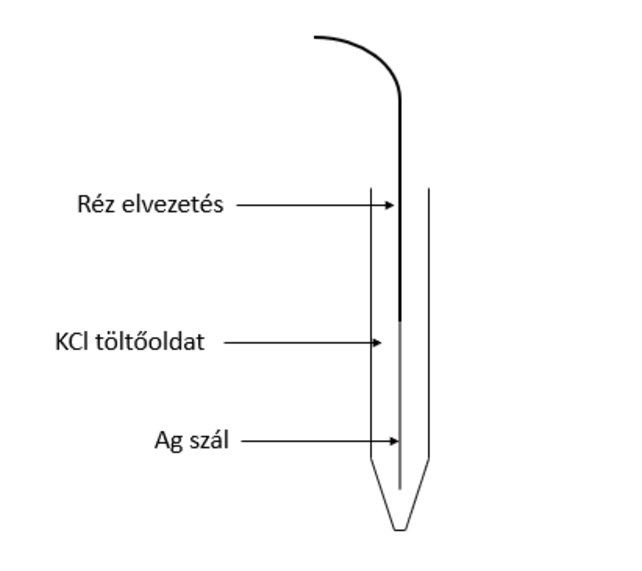
\includegraphics[width=0.5\textwidth]{img/electrode1.eps}
\caption{Az általam készített mikroméretű referencia elektród fotója (bal oldal) és sematikus ábrája (jobb oldal)}
\label{fig:electrode}
\end{figure}

\section{Céltárgyak}

Laboratóriumi munkám során kétféle céltárgyat alkalmaztam: egy jól jellemzett grafit céltárgyat és egy vas-cink galvánpárt. Mindkét céltárgy epoxi gyantába volt öntve, így a grafit és fémminta egy meghatározott része érintkezett az oldattal. Az epoxi gyanta alsó részén rézdrótok által volt megoldva az elektromos elvezetés. Minden mérés előtt és után, a céltárgyak felületét políroztam, csiszolópapír (1000 $\upmu$m, 2000 $\upmu$m majd 4000 $\upmu$m szemcseméretű Al$_2$O$_3$) segítségével. Ezután, hogy a cellát létrehozzam és oldatot öntsek a felületére a mintának, hézagmentesen körbetekertem átlátszó ragasztószalaggal, úgy hogy körülbelül fél centiméterrel magasabban legyen a céltárgy felületétől. A céltárgyak felszínét vízszintbe állítottam minden mérés előtt, ehhez egy buborékos vízszintezőt használtam. Így a pásztázás síkja párhuzamos volt a céltárgy X-Y síkjával. A cella létrehozásához szükséges oldatként a laboratóriumban található desztilláló készülék (Elix® Essential 10 Water Purification System, Milli-Q, Progard® TS2, PR0G0T0S2) által előállított desztillált vizet használtam, melynek vezetése 0,067 $\upmu$S/cm volt. Ez utóbbi adatot a készülék szolgáltatta szintén. 

\section{Mikroszkóp és a mérőprogram}

A mérésekhez egy, a tanszéken a közelmúltban épített pásztázó elektrokémiai mikroszkópot (Eppendorf MIM4 Micromanipulator), valamint egy nagy bemeneti impedanciájú mérőműszert (eDAQ QUAD MF isoPod 452) használtam, mely utóbbit a témavezetőm által készített program vezérelt. Szükségem volt továbbá még egy nagyméretű stacioner referencia elektródra (Radiometer Electrodes, K401 Kalomel, SE-2), melyhez képest a mikroméretűvel mértem a potenciált a cellában. Ezt a pásztázási területen kívül helyeztem el, hogy a méréseket ne zavarja. 

Kétféle pásztázási algoritmust használtam, horizontális, a minta felületének síkjával párhuzamos 2D pásztázást, és a minta felületének síkjára merőleges 2D pásztázást. Az X és Y irányú lépésköz 100 $\upmu$m volt minden esetben. A teljes pásztázott terület a mintától függött, melyről a mérési eredmények ismertetése során írok részletesen. A mikroelektród mozgatási sebessége két szomszédos mérési pont között 1000 $\upmu$m/s volt. Minden egyes mérés előtt 0.2 s várakozási időt adtam meg, hogy a mozgatást követően egy közel egyensúlyi, stabil potenciálérték kialakulhasson.  

Mivel az elektromos mező Z irányú komponenséhez vertikális potenciálkülönbség mérésekre van szükség, a horizontális pásztázásokat kétszer végeztem el, bizonyos Z irányú eltolással, melyet az egyes mérések bemutatásánál adok meg.

A mérések előtt a Z referencia koordinátát is szükséges volt rögzítenem. A poteniometriás méréseknél ismeretes, hogy a Z koordináta beállítása nehézségekbe ütközik \cite{klucsikmsc}. Az említett szakdolgozó az \emph{Irodalom} részben általam is megemlített visszacsatolás jelenségét alkalmazta a probléma kiküszöbölésére. Könnyen polarizálható, kis ellenállású volfrám mikroelektródokat használt amperometriás üzemódban, ismerve a pontos elektród átmérőt és a távolságot, melyekkel kiszámítható ez a komponens. Mivel ezen esetben erre nem volt lehetőségem a feedback hiányában, illetve a kapillárisom nyitott végű volt, én ezt a következőképpen oldottam meg: miután elhelyeztem a mikroméretű referencia elektródot a mikroszkóp foglalatába, elkezdtem közelíteni az adott céltárgy felületéhez, annak a galvánpár közötti középpontja felé. Mikor szemmel láthatólag közel volt a felülethez, kis mértékben közelítettem, majd mozgattam minimálisan a céltárgyat, hogy az elektród a felülettel együtt mozog-e. Ha nem, még közelítettem, hogy ütközésig érjen hozzá. Amikor ezt elértem, 0 mikrométernek tekintettem ezt, és innentől számítva adtam meg a programnak, hogy hány mikrométerrel a céltárgy felett mozogjon Z irányban. Így, mint említettem korábban, a pásztázási terület középpontjában volt az elektród. Viszont a program meanderezve haladt, jobbról balra, majd ugrott egyet a következő pásztázási vonal jobb oldalára újra.  Emiatt a teljes pásztázási terület ½ értékével léptem, tehát X/2 és Y/2 értékkel, hogy eljussak a mérés kezdőpontjába. Ezen a ponton lenulláztam a programot, hogy referencia kezdőpontként alkalmazzam a mérésekhez.

\section{Mérések kiértékelése}

Az elektromos mező kiszámításához kétféle módszer állt rendelkezésemre, az analitikus és numerikus. Előbbi esetében ismernünk kellene az f(x) függvényeit a méréseknek, melyeket deriválnánk. Ez azonban túl bonyolult és időigényes lenne. Emiatt a numerikus deriválást választottam, az \emph{Irodalom} című fejezetben leírt \ref{eq:nabla}. egyenlet alkalmazásával. A mérések eredményeképp kapott potenciáltértképeket először deriválnom kellett hely szerint. Az adatfájlokat egyenként importáltam a Qti Plot nevű programba, egy X-Y-E oszlopokból álló táblázatba. X és Y oszlopok tartalmazták a mérések lépéseit, E pedig a mért potenciálértéket. Ezután a potenciálértékek oszlopát mátrixszá alakítottam, a pásztázási területekkel arányos oszlop és sor számúra. Grafit minta esetében a vertikálisnál 51 oszlopos 11 soros, horizontális mérésnél 41 oszlopos és 31 soros mátrixot kaptam. A vas-cink céltárgynál vertikális mérésnél 31 oszlopos és 11 soros az anód és katód esetén is, horizontálisan pedig egyet-egyet az anód és katód oldaláról, amik 31 oszlopot és 21 sort tartalmaztak. 

Az így kapott mátrixoknak Excelben X-Y irányba kiszámoltam a cellák közti különbségét. Vagyis a táblázat egy adott potenciálértéke alatti és feletti, illetve két oldali értékek különbségét. Ez a mátrixok szélén nehézségekbe ütközött, mivel nem volt számpár, aminek a differenciálját vehettem volna. Ezért a mátrixot tükröztem, mivel így különbségük nulla. Tehát a szélső differenciált nullának vettem X és Y komponens esetében is. Végül elosztottam a két mérés közti távolsággal (Z komponens) a kapott értékeket. Megkaptam az X, Y és Z komponenseket, melyeket bevittem mátrixként ismét a Qti Plot programba. Ily módon megkaptam az X-Y-Z komponensek mátrixát.

Következő lépésben a mátrixokat visszaalakítottam táblázatos formába, mely három oszlopos volt, az első kettő a mérés paraméterei, a harmadik pedig a számolt komponensek külön-külön táblázatban. Ezekből a táblázatokból pedig az X-Y-Z számolt komponenseket, vagyis a harmadik oszlopot importáltam az eredeti táblázatba, így kaptam összesen hat oszlopot. Illetve a horizontális pásztázások esetén be kellett szúrnom még egy hetedik oszlopot, ami csupa 0 értékeket tartalmazott. Ez a Gnuplot-al való ábrázolásomhoz volt szükséges, mivel a programnak a 3D-os ábrázoláshoz meg kellett adnom egy Z paramétert is az X és Y mellett. 

Hogy az elektromos mező értékét megkapjam, alkalmaztam az \emph{Irodalom} fejezetben leírt \ref{eq:field1}. egyenletet. Tehát megszoroztam a számolt komponenseket az adott mérések közti távolsággal. A $\frac{\partial E}{\partial x}$ értelmében ez ugyanazt az eredményt adja, mintha osztást végeznék, a mértékegységek figyelembevételével. Az áramsűrűség ábrázolásához ezeket az oszlopokat még a víz fajlagos vezetőképességével is meg kellett szoroznom. Az ábrázoláshoz a Z komponens oszlopainak áramértékét nulláznom kellett, mivel nem valós értékeket mutattak. Az epoxi gyanta felett is nullától különböző értéket kaptam, viszont itt nem játszódik le se oxidáció, se redukció. Ez annak tulajdonítható, hogy a két mérés közt jelentős idő telt el, ami elég a potenciálváltozáshoz. Vagyis az elektród potenciálja időben változott.
